\section{Transaktionseigenschaften}

\subsection{ACID}
\textit{ACID} ist ein Akronym, welches häufig verwendet wird, um Eigenschaften auszudrücken, die eine Transaktion auf Datenbankebene aufweisen sollte. Die Buchstaben stehen für \textbf{A}tomicity (Atomarität), \textbf{C}onsistency (Konsistenz), \textbf{I}solation (Isolation) und \textbf{D}urability (Dauerhaftigkeit)\cite{Dey.}. 

\paragraph*{Atomarität} \mbox{} \\
Eine Transaktion, also eine Folge von Datenbankoperationen, muss entweder alle Operationen ausführen oder in einem Fehlerfall alle Änderungen auf den ursprünglichen Zustand zurückrollen. 

\paragraph*{Konsistenz} \mbox{} \\
Alle Änderungen der Datenbank überführen die Daten von einem konsistenten Zustand in einen ebenfalls konsistenten Folgezustand. 

\paragraph*{Isolation} \mbox{} \\
Isolation stellt sicher, dass sich parallel in Ausführung befindliche Transaktionen nicht gegenseitig beeinflussen können. Das bedeutet, dass eine Transaktion Teile der Datenbasis sperren können muss. Eine solche Sperre führt jedoch zu blockierendem Verhalten und schränkt somit die nebenläufige Benutzung der Datenbank ein. 

\paragraph*{Dauerhaftigkeit} \mbox{} \\
Dauerhaftigkeit von Transaktionen muss gewährleistet sein, damit bei einem Ausfall Transaktionsdaten nicht verloren gehen. Um Dauerhaftigkeit zu erreichen, wird ein Transaktionslog gefährt, welches im Ausfall verwendet werden kann, um die verlorenen Transaktionen nachzuspielen. 

\subsection{BASE}
Als Alternative zum Konsistenzmodell \acrshort{acid} soll nun \acrshort{base} (\textbf{B}asically \textbf{A}vailable, \textbf{S}oft State, \textbf{E}ventual Consistency) vorgestellt werden. BASE ist schwächer als ACID, verfolgt jedoch ebenfalls die Wahrung der Konsistenz in einem System. Es kommt am häufigsten in NoSql-Datenbank zum Einsatz, die die Daten hauptsächlich in Aggregaten zusammenfassen. Innerhalb eines Aggregats können Daten transaktionell verändert werden. Transaktionen über die Daten mehrerer Aggregate werden jedoch nicht atomar sondern sequentiell ausgeführt. Dabei kann das System die Ausführung der Commits der Teilschritte unter hoher Last aufschieben und zu einem späteren Zeitpunkt durchführen. Dadurch erreichen Datenbanksysteme mit BASE-Eigenschaften eine höhere Erreichbarkeit. Diese hohe Erreichbarkeit wird eingetauscht für Atomarität und strenge Konsistenz\cite{SadalagePramodJ.andFowlerMartin.2012}. 

\paragraph*{Grundsätzlich verfügbar (BA)}\mbox{}\\
Das System ist hochverfügbar. Trotz hoher Last beantwortet das System Anfragen. Die Antworten können unter Umständen einen intermediären Zustand abbilden, der inkonsistent ist. 

\paragraph*{Weicher Zustand (S)}
Bevor alle Operationen einer Transaktion ausgeführt wurden, befindet sich das System in einem Übergangszustand. Dieser Übergangszustand kann Konsistenzfehler aufweisen. In Bezug auf ACID verletzt dieser \textit{Soft State} die Atomarität und die Isolation.

\paragraph*{Schlussendliche Konsistenz (E)}
Als schlussendlich konsistent wird das System angesehen, wenn alle Teiloperationen aller Transaktionen abgeschlossen sind. Der Zustandsübergang beginnt in einem konsistenten Zustand, geht in einen inkonsistenten \textit{Soft State} über und befindet sich nach Abschluss aller Teiloperationen in einem konsistenten Endzustand. 

\subsection{CAP-Theorem} \label{subsec:cap-theorem}
Das CAP-Theorem wurde \citeyear{Brewer.} in einem Vortrag auf dem PODC Symposium von \citeauthor{Brewer.} vorgestellt. Darin behauptete \citeauthor{Brewer.} folgende Aussage:

\begin{theorem}[CAP-Theorem] 
Für einen Webservice ist es unmöglich, folgende drei Eigenschaften zu garantieren:
\begin{itemize}
	\item Konsistenz (Consistency)
	\item Verfügbarkeit (Availability)
	\item Partitionstoleranz (Partition-tolerance)
\end{itemize}
Alle drei Eigenschaften sind erwünschenswert und werden von realen Webservices erwartet\cite{Brewer.}.
\end{theorem}

Der Beweis für dieses Theorem wurde \citeyear{Gilbert.2002} von \citeauthor{Gilbert.2002} bewiesen. Das CAP-Theorem ist in \cref{fig:cap_theorem} dargestellt. Von den drei Möglichkeiten sind nur zwei realisierbar. In einem verteilten System ist die Partitionstoleranz bereits inbegriffen, weshalb die Wahl zwischen Konsistenz und Verfügbarkeit besteht. 

\begin{figure}[!htbp]
	\centering
	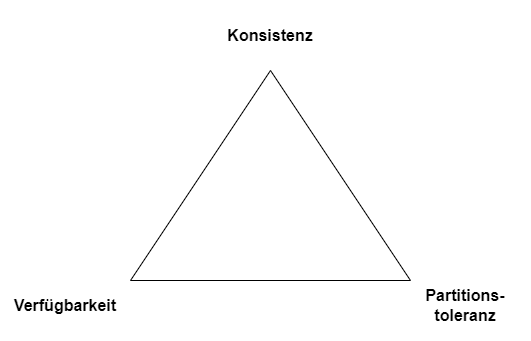
\includegraphics[height=5cm]{figures/ChapterGrundlagen/cap_theorem.png}
	\caption{Visuelle Darstellung des CAP-Theorems}
	\label{fig:cap_theorem}
\end{figure}
\FloatBarrier

Das Theorem kann dazu verwendet werden, ein verteiltes System in verschiedene Kategorien zu unterteilen. 

\paragraph*{AP-System} \mbox{} \\
AP-Systeme setzen auf Verfügbarkeit und Partitionstoleranz. Ein Beispiel dafür ist ein soziales Netzwerk. Es ist annehmbar, wenn neue Beiträge nicht live sondern leicht verzögert angezeigt werden. Besteht eine Netzwerkpartition, ist das System trotzdem funktional, arbeitet unter Umständen auf inkonsistenten Daten. Das bedeutet, dass in der einen Partition ein neuer Beitrag angezeigt wird, in der anderen Partition ist dieser Beitrag noch nicht synchronisiert und kann demnach nicht angezeigt werden. Das System ist inkonsistent. Unverfügbarkeit ist für ein soziales Netzwerk jedoch wesentlich schlimmer als ein inkonsistentes System, weshalb solche Anwendung oft als AP-System realisiert werden.

\paragraph*{CP-System} \mbox{} \\
Transaktionskritische Systeme, die unter keinen Umständen einen inkonsistenten Zustand erreichen dürfen, sind als CP-System umgesetzt. Dabei wird die Verfügbarkeit im Falle von Netzwerkpartitionen nicht gewährleistet. 

\section{Isolationsanomalien}
Werden Systeme durch mehrere Benutzer und somit durch mehrere Transaktionen gleichzeitig verändert, können verschiedene Anomalien auftreten. Diese Anomalien könnnen inkonsistente Datenbankzustände verursachen. Die Anomalien treten dann auf, wenn im Mehrbenutzerbetriebs mehrere gleichzeitig in Ausführung befindliche Transaktionen auf dieselben Ressourcen zugreifen. 

\subsection{Anomalien} \label{subsec:isolationsanomalien}
\paragraph*{Dirty Reads} \mbox{} \\
Dirty Reads treten auf, wenn eine Transaktion einen Datensatz modifiziert und eine zweite Transaktion diese liest, bevor die Änderungen committet wurden. Rollt die erste Transaktion die Änderungen zurück, hat der zweite Prozess nicht existierende Daten gelesen\cite{IBMDocumentation.2021}.

\paragraph*{Lost Updates} \mbox{} \\
Lost Updates treten auf, wenn zwei Transaktionen gleichzeitig den selben Datensatz updaten\cite{IBMDocumentation.2021}.

\paragraph*{Non Repeatable Read} \mbox{} \\
Nonrepeatable Reads treten auf, wenn wiederholte Lesevorgänge einer Transaktionen unterschiedliche Ergebnisse liefern. Dies tritt auf, wenn die gelesenen Datensätze von einer anderen Transaktion verändert wurden\cite{IBMDocumentation.2021, PostgreSQLDocumentation.2023}.

\paragraph*{Phantom Read} \mbox{} \\
Phandomreads treten auf, wenn eine Transaktion eine Menge an Datensätzen mit einer bestimmten Suchbedingung mehrfach abfragt. Die Abfrageergebnisse verändern sich, wenn die Menge der Suchbedingung erfüllenden Datensätze durch eine andere Transaktion verändert wurde\cite{PostgreSQLDocumentation.2023}. 

\subsection{Isolationsstufen}
Implementierungen des \acrshort{dbms} lösen dieses Problem häufig über die Isolationsstufen \textit{READ\_UNCOMMITTED}, \textit{READ\_COMMITTET}, \textit{REPEATABLE\_READ} und \textit{SERIALIZABLE}. \textit{READ\_UNCOMMITTED} ist die niedrigste und \textit{SERIALIZABLE} die höchste Isolationsstufe. Wählt eine Transaktion eine Isolationsstufe aus, werden für die Dauer der Transaktion Ressourcen gesperrt. Je höher die Stufe, desto mehr Ressourcen werden gesperrt. Deshalb führt die Verwendung einer höheren Isolationsstufe zu einem geringeren Performance, da Transaktionen öfter abgelehnt werden und zurückgerollt werden müssen\cite{Zeleny.20220601}. 
